\section{Diseño del proyecto}\label{sec:diseno}

\subsection{Análisis del problema y de los datos}\label{sec:obtencion}

Considerando que los datos contenidos en los archivos con formato \gls{bil} contienen 168 columnas con información de las diferentes longitudes de onda\ \cite{WhatIsHy18:online} y además el nivel de contaminación \gls{don} de cada grano, podemos generar un \gls{dataset} con los datos de cada grano, haciendo la media de cada longitud de onda por cada píxel del mismo grano. Una vez hemos extraído la información de todos los archivos \gls{bil} y la hemos guardado en un archivo \acrshort{csv}, podemos entrenar los modelos sobre este.

\subsection{Preprocesado de datos}\label{sec:preprocesado}

Ahora que tenemos los datos en un solo archivo \acrshort{csv}, el siguiente paso es preprocesarlos. Para ello, hemos realizado los siguientes pasos: 

\begin{enumerate}
    \item Eliminación de columnas
    \item Codificación
    \item Valores atípicos (\textit{outliers})
    \item Separación en datos de entreno y de prueba (\textit{train-test-split})
    \item Balanceo de datos
    \item Preprocesado común, (\textit{pipeline})
    \begin{enumerate}
        \item Separación de datos aplicando la primera derivada 
        \item Aumento de dimensionalidad (\textit{Polynomial Features})
        \item Estandarización  (\textit{Standard Scaler})
        \item Reducción de dimensionalidad (\textit{Principal Component Analysis})
    \end{enumerate}
    
\end{enumerate}


\subsubsection{Eliminación de columnas, codificación y valores atípicos}

Existen datos que nos interesan como medida de seguridad, pero no nos interesa que un modelo entrene con ellos, ya que podría inferir patrones irreales o incluso memorizarlos. En nuestro caso, un ejemplo sería una columna que indicase el número identificador del grano o el archivo del cual se han extraído los datos.

La codificación consiste en transformar columnas con datos categóricos en columnas de datos numéricos, pues los modelos de \acrshort{ml} funcionan mejor con valores numéricos. En nuestro caso, la única columna con valores no numéricos era la columna de la contaminación, que podía tomar los valores \textit{\{B, C\}}, así que lo codificamos manualmente como se muestra a continuación:

{
    \centering
    \textit{B \longrightarrow{} 0}, \textit{C \longrightarrow{} 1}\par
}

Los valores atípicos u \textit{outliers} son aquellos valores inusuales en los datos que pueden distorsionar nuestros análisis estadísticos. Sin embargo, se debe tener en cuenta que puede haber mucha variación en la naturaleza de nuestro problema. Por ello, se deben diferenciar los \textit{outliers} que se pueden incluir en los datos y los que no. En nuestro caso, no hemos quitado ningún \textit{outlier}, pues la mayoría de granos tenía alguna columna de datos que no entraba dentro de lo ``normal'', como por ejemplo se puede observar en la \textit{Figura\ \ref{fig:outliers}}. Por lo que después de probar a quitar todos los granos que alguna de sus columnas fuera un \textit{outlier} (con el \textit{Código\ \ref{code:zscore}}), nos quedamos sin datos.

\begin{figure}[!h]
    \centering
    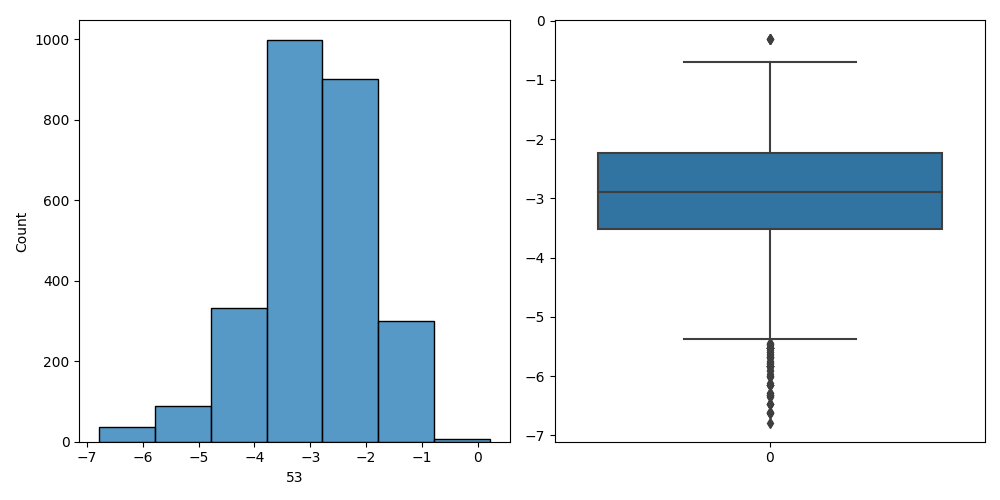
\includegraphics[width=0.7\linewidth]{media/images/col-53-outliers.png}
    \caption{Representación de los \textit{outliers} de la columna 53 en un gráfico de velas, fuente propia, \textit{Código\ \ref{code:plot-outliers}}}\ \label{fig:outliers}
\end{figure}


\subsubsection{Separación de datos de entreno y de prueba}

En todo el proyecto hemos estado utilizando la librería \href{https://scikit-learn.org/stable/}{sklearn}, esta tiene un submódulo con una función \href{https://scikit-learn.org/stable/modules/generated/sklearn.model_selection.train_test_split.html}{sklearn.model\_selection.train\_test\_split} para separar el \gls{dataset} en entreno y prueba. De esta función, lo más importante es que nos permite la opción de utilizar \textit{stratify}, la cual es muy recomendable cuando el \textit{dataset} no está balanceado.

De todas las opciones, cabe resaltar una que hemos habilitado, pues como en el \gls{dataset} original las etiquetas no están balanceadas y hay muchos más granos sanos que contaminados, es importante que los granos contaminados estén igualmente representados tanto en el conjunto de prueba como en el de entreno, esto se consigue con la opción \textit{stratify}.


\subsubsection{Balanceo de datos}\ \label{sec:balance}

Podemos ver en la \textit{Figura\ \ref{fig:unbalance}} que los datos no están balanceados, es decir, que la columna que nos interesa `Contaminación' no tiene un número de datos similares en cada clase. En nuestro caso, como en general es más complicado encontrarse un grano contaminado, tenemos más granos sanos.

\begin{figure}[!h]
    \centering
    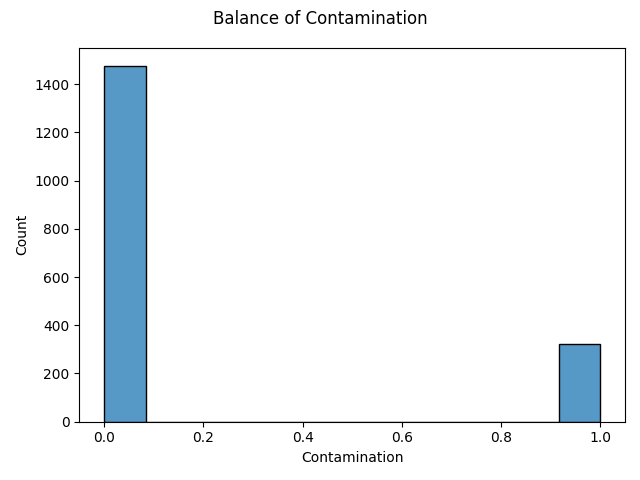
\includegraphics[width=0.5\linewidth]{media/images/unabalance.png}
    \caption{Balanceo de la clase objetivo del \gls{dataset}, fuente propia}\ \label{fig:unbalance}
\end{figure}

Al tener las clases desbalanceadas tenemos varias opciones:
\begin{enumerate}
    \item Usar métodos de evaluación que tengan en cuenta el desbalance de las clases.
    \item Balancear el \gls{dataset} utilizando tanto \textit{undersampling} como \textit{oversampling}.
\end{enumerate}

La toma de nuevos datos es costosa y como tenemos relativamente pocos para la cantidad de columnas (las 168 longitudes de onda), el balanceo de datos es esencial. Sorteamos este problema utilizando métricas que tienen en cuenta el balance de los datos. Sin embargo, podemos balancear los datos en dos pasos: \textit{undersampling} y \textit{oversampling}. 

Como su nombre indica, \textit{undersampling} es una técnica para reducir las muestras de la clase mayoritaria, en nuestro caso los granos sin contaminar. Existen varias técnicas para hacer \textit{undersampling}, las cuales comentaremos en la \textit{Sección\ \ref{sec:undersampling}}. Por otro lado, el \textit{oversampling} consiste en la creación de datos sintéticos, similares a los reales, para suplir la diferencia de balanceo entre las diferentes clases. Al igual que con el \textit{undersampling}, existen diversas técnicas que comentaremos más adelante en la \textit{Sección\ \ref{sec:oversampling}}.

\paragraph{Undersampling}\ \label{sec:undersampling}


A la hora de balancear los datos, buscamos, de alguna forma, reducir la diferencia en el número de muestras en las diferentes clases del dataset. En el paso de \textit{undersampling}, buscamos reducir la cantidad de muestras de las clases mayoritarias. Para ello, debemos de alguna forma determinar qué muestras de las clases mayoritarias son más redundantes para evitar eliminar muestras `críticas'. Para ello hemos decidido utilizar los algoritmos de la librería \href{https://imbalanced-learn.org/stable/}{imblearn} que fue diseñada específicamente para los problemas de clasificación sobre \textit{datasets} desbalanceados.\ \cite{3Undersa98:online}

El primer algoritmo que probaremos será \textit{RandomUnderSampler}, el cual consiste en seleccionar un subconjunto aleatorio de datos. Para intentar no eliminar datos importantes como hemos comentado antes, hay otra versión que aplica una de las tres versiones de la heurística \textit{NearMiss}\ \cite{3Undersa98:online}, la cual se basa en el algoritmo \textit{nearest neighbors}:

\begin{enumerate}
    \item La versión \textbf{NearMiss1} elimina aquellos datos cuya distancia media a sus \textit{N} vecinos más cercanos de la clase minoritaria sea menor.
    \item La versión \textbf{NearMiss2} es parecida a la \textbf{1}, pero en esta la distancia media se computa sobre los \textit{N} vecinos más lejanos de la clase minoritaria.
    \item La versión \textbf{NearMiss3} consta de dos pasos, primero, de cada elemento de la clase minoritaria selecciona los \textit{M} vecinos más cercanos de la clase mayoritaria. Luego, por cada muestra seleccionada se calcula la distancia media respecto a los \textit{N} vecinos más cercanos de la clase minoritaria y se eliminan los que, de media, estén más alejados.
\end{enumerate}

El siguiente algoritmo, \textit{Tomek Links}, detecta los llamados \textit{Tomek Links}, estos son enlaces entre dos muestras de diferente clase, pongamos \(x\) e \(y\), definidos tal que para cualquier muestra \(z\): 
\[d(x,y) < d(x,z)\ and\ d(x,y) < d(y,z)\], donde \(d(a, b)\) es la distancia entre la muestra \(a\) y \(b\). En resumen, un \textit{Tomek Link} se da entre las muestras de distintas clases más cercanas entre sí. Este algoritmo suele ser bueno a la hora de eliminar ruido en los datos.

Por último, el algoritmo \textit{Edited Nearest Neighbours} elimina las muestras que no se parezcan demasiado a sus vecinos\ \cite{Wil72}. Para ello, comprueba para cada muestra que sus \textit{N} vecinos más cercanos sean de su misma clase, si no se cumple,podemos elegir si nos quedamos con las muestras de la clase mayoritaria o si eliminamos todas las muestras.


\paragraph{Oversampling}\ \label{sec:oversampling}

El segundo paso es el \textit{oversampling}, el cual consiste en la creación de los datos sintéticos para suplir la carencia de datos de las clases minoritarias. Al igual que en el paso anterior, hay algoritmos para realizar estas técnicas implementados en la librería \textit{imblearn}, sin embargo preferimos utilizar \href{https://sdv.dev/}{The Synthetic Data Vault} \cite{Synthesi69:online}, pues tiene mejor documentación y tiene un método sencillo para evaluar los datos generados. 

En la librería hay los siguientes cuatro sintetizadores de datos:

\begin{enumerate}
    \item \textit{Gaussian Copula Synthesizer} \cite{Gaussian4:online}, el cual utiliza métodos estadísticos clásicos.
    \item \textit{TVAESynthesizer} \cite{TVAESynt0:online}, basado en \textit{VAE} \cite{Variatio61:online}, utiliza técnicas de redes neuronales.
    \item \textit{CTGANSynthesizer} \cite{CTGANSyn50:online} y \textit{CopulaGAN} \cite{CopulaGA37:online}, ambos utilizan métodos de \textit{deep learning} basados en \textit{GAN} \cite{Generati72:online}, los comentamos por encima pues no los probaremos porque no son recomendables para datasets con tantas columnas no discretas, pues generarían un dataset con muchísimas más columnas (en nuestro caso, multiplicarían las columnas por once, es decir, tendríamos 1848). 
\end{enumerate}

Una vez aumentado el dataset con los datos sintéticos, evaluaremos cuál es mejor para nuestro problema comparando la similitud de los datos generados con los reales y la calidad de los modelos resultantes de entrenar con el nuevo dataset.


\subsubsection{Preprocesado común}

Después de balancear los datos, debemos modificarlos para que tengan algunas propiedades que suelen ser preferibles a la hora de entrenar ciertos modelos. Es decir, hay modelos que les vendrá mejor tener los datos estandarizados, por ejemplo, y otros que no hará falta o será contraproducente, al final será la experiencia lo que nos diga qué pasos son preferibles.

Antes de comentar las diferentes formas de preprocesado de los datos, hemos preparado un entorno para entrenar una batería de modelos distintos sobre estos para ver y comparar su efectividad. Esta comparación de los modelos resultantes la haremos con las métricas que hemos comentado anteriormente.


Los pasos que hemos probado para preprocesar los datos son los que comentamos en las siguientes secciones.

\paragraph{Primera derivada}

Un primer paso recomendado desde el laboratorio, ya que era lo que utilizaban ellos en su modelo estadístico, es aplicar la primera derivada. El hacerlo permite mínimamente separar los granos contaminados de los que no, pues aplicar la derivada suaviza los datos, eliminando parte del ruido y dejando solo las tendencias como podemos ver en la \textit{Figura\ \ref{fig:derivative}}.
De todas formas, probaremos que este paso sea realmente útil haciendo pruebas con y sin él.

\begin{figure}
    \centering
    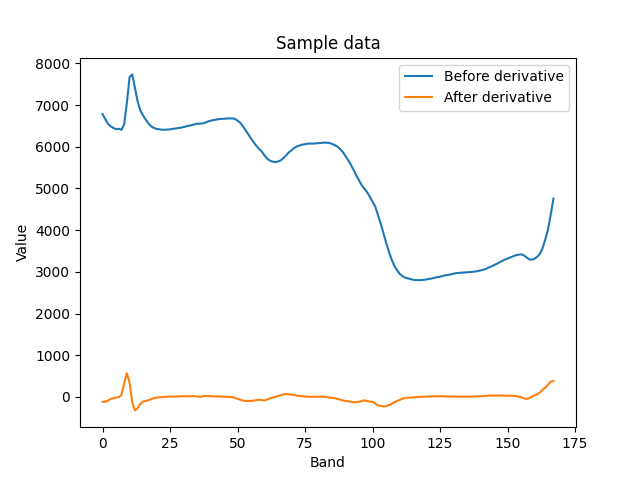
\includegraphics[width=0.8\linewidth]{media/images/derivative.png}
    \caption{Comparación de aplicar la primera derivada sobre la primera muestra. Fuente propia}\ \label{fig:derivative}
\end{figure}

\paragraph{Transformada}

El siguiente paso que podemos probar es aplicar la transformada, como los resultados habiendo derivado los datos son mejores, transformaremos los datos después de derivarlos. La transformada consiste en transformar cada columna para que tengan una forma gaussiana\ \cite{sklearnp39:online}, a continuación mostraremos por qué, a grandes rasgos, esta forma es interesante. \cite{TheRoleo87:online}

\begin{enumerate}
    \item \textit{Realismo}, en muchos problemas con datos reales, la distribución de los datos es gaussiana.
    \item \textit{Propiedades estadísticas}, la forma de campana (o gaussiana) tiene propiedades conocidas que permiten la aplicación de varias técnicas estadísticas.
    \item \textit{Compatibilidad}, muchos modelos estadísticos y de \gls{ml} asumen que los datos tienen una distribución gaussiana.
\end{enumerate}

Como estamos utilizando \textit{sklearn}, tenemos una clase que nos aplica la transformada \href{https://scikit-learn.org/stable/modules/generated/sklearn.preprocessing.PowerTransformer.html}{sklearn.preprocessing.PowerTransformer}, por defecto esta clase además te aplica una estandardización de los datos, pero la hemos deshabilitado para aplicarla en el siguiente paso. 


\paragraph{Estandarización}

A continuación, probaremos la estandarización de los datos como hemos comentado anteriormente. Utilizaremos la clase \href{https://scikit-learn.org/stable/modules/generated/sklearn.preprocessing.StandardScaler.html}{sklearn.preprocessing.StandardScaler}. La estandardización consiste en el centrado y escalado de los datos. Para ello, columna por columna, restamos la media de los valores (centramos en torno al 0) y los dividimos por la varianza (para que la desviación tienda a 1). Tener los datos estandarizados suele ser un requisito para obtener buenos resultados al entrenar algunos modelos.\ \cite{sklearnp24:online}


\paragraph{Disminución y aumento de dimensionalidad}

Por último, podemos probar dos pasos que suelen ir juntos. El primero, \href{https://scikit-learn.org/stable/modules/generated/sklearn.preprocessing.PolynomialFeatures.html}{sklearn.preprocessing.PolynomialFeatures}, nos permite generar nuevas columnas de datos que consisten en combinar las demás columnas, multiplicándolas entre sí y elevando a un grado específico (segundo grado en nuestro caso). De esta forma, de nuestro \gls{dataset} de 168 columnas, obtenemos uno de 14365 columnas. Por ello, debemos aplicar el segundo y último paso para reducir la dimensionalidad de los datos y poder entrenar modelos en un tiempo razonable. Este paso es \href{https://scikit-learn.org/stable/modules/generated/sklearn.decomposition.PCA.html}{sklearn.decomposition.PCA} o \textit{Principal Component Analysis}, el cual reduce la dimensionalidad proyectando los datos a una espacio de menor dimensionalidad. Podemos leer algo más al respecto sobre \textit{PCA} en \ \cite{Principa62:online}. 